Expanding the given equation, we have,
\begin{align}
    x^2 -8xy +16y^2 -51y =0 \label{eq:solutions/41/1/eq:1}
\end{align}
The general equation of second degree is given by
\begin{align}
	ax^2+2bxy+cy^2+2dx+2ey+f=0 \label{eq:solutions/41/1/gen_eq}
\end{align}
and can be expressed as
\begin{align}
	\vec{x}^T\vec{V}\vec{x}+2\vec{u}^T\vec{x}+f=0 \label{eq:solutions/41/1/conic_eq}
\end{align}
where
\begin{align}
	\vec{V} &= \vec{V}^T = \myvec{a & b \\ b & c}
	\\
	\vec{u}^T &= \myvec{d & e}
\end{align}
From equation \eqref{eq:solutions/41/1/eq:1} , we get
\begin{align}
	\vec{V} &= \myvec{1 & -4\\-4 & 16}\label{eq:solutions/41/1/eq:2}\\
	\vec{u} &= \myvec{0\\-\frac{51}{2}}\label{eq:solutions/41/1/eq:3}\\ 
	f &= 0 \label{eq:solutions/41/1/eq:4}
\end{align}
Expanding the determinant of $\vec{V}$ we observe, 
\begin{align}
	\mydet{1 & -4\\-4 & 16} = 0
\end{align}
Therefore, \eqref{eq:solutions/41/1/eq:1} is a parabola.

The characteristic equation of $\vec{V}$ is given as follows,
\begin{align}
		\mydet{\lambda\vec{I}-\vec{V}} = \mydet{\lambda-1&4\\ 4&\lambda-16} &= 0\\
		\implies \lambda^2-17\lambda &= 0\label{eq:solutions/41/1/eq:5}
\end{align}
The eigenvalues are given by
\begin{align}
		\lambda_1=0, \lambda_2=17\label{eq:solutions/41/1/eq:6}    
\end{align}
For $\lambda_1 = 0$, the eigen vector $\vec{p}$ is given by 
\begin{align}
		\vec{V}\vec{p} = 0
\end{align}

Row reducing $\vec{V}$ 
\begin{align}
		\myvec{1&-4\\-4&16}\xleftrightarrow[R_2=R_2+R_1]{R_2=R_2/4}\myvec{1&-4\\0&0}\\
		\implies\vec{p}_1=\frac{1}{\sqrt{17}}\myvec{-4\\-1} \label{eq:solutions/41/1/eq:7}
\end{align}
Similarly, 
\begin{align}
		\vec{p}_2=\frac{1}{\sqrt{17}}\myvec{-1\\4} \label{eq:solutions/41/1/eq:8}
\end{align}

Thus,
\begin{align}
		\vec{P}&=\myvec{\vec{p_1}&\vec{p_2}}=\frac{1}{\sqrt{17}} \myvec{-4 & -1\\ -1 & 4} 
\end{align}
The equation of the parabola is:
\begin{align}
		\vec{y^T}\vec{D}\vec{y}&=-2\eta\myvec{1&0}\vec{y}
\end{align}
where
\begin{align}
		\eta=\vec{u}^T\vec{p_1}=\frac{51}{2\sqrt{17}}
\end{align}
and focal length of the parabola is given by 
\begin{align}
	\frac{\abs{2\vec{u}^T\vec{p_1}}}{\lambda_2}	= \frac{3}{\sqrt{17}}
\end{align}

Now,
\begin{align}
		\myvec{\vec{u^T}+\eta\vec{p_1^T} \\ \vec{V}}\vec{c}=
		\myvec{-f \\ \eta\vec{p_1}-\vec{u}} \label{eq:solutions/41/1/eq:9}
\end{align}
using equations \eqref{eq:solutions/41/1/eq:2}, \eqref{eq:solutions/41/1/eq:3} and \eqref{eq:solutions/41/1/eq:9}
\begin{align}
	\myvec{-6& -27 \\ 1 & -4 \\  -4 & 16 }\vec{c}=\myvec{0 \\ -6\\ 24} 
\end{align}

Forming the augmented matrix and row reducing it:
\begin{align}
		\myvec{-6 & -27 & 0\\1 & -4 & -6 \\-4 & 16 & 24}\\
		\xleftrightarrow[]{R_3\leftarrow R_3+ 4R_2} 
		\myvec{-6 & -27 & 0\\1 & -4 & -6 \\0 & 0 &0 }\\
		\xleftrightarrow[]{R_1\leftarrow R_1/(-6)} 
		\myvec{1 & 9/2 & 0\\1 & -4 & -6\\0 & 0 &0 }\\
		\xleftrightarrow[]{R_2\leftarrow R_2-R_1} 
		\myvec{1 & 9/2 & 0\\0 & -17/2 & -6 \\0 & 0 &0 }\\
		\xleftrightarrow[]{R_2\leftarrow (-\frac{2}{17})R_2}
		\myvec{1 & 9/2 & 0\\0 & 1 & 12/17\\0 & 0 &0}\\ 
		\xleftrightarrow[]{R_1\leftarrow R_1 -(\frac{9}{2})R_2}
		\myvec{1 & 0 & -54/17\\0 & 1 & 12/17 \\0 & 0 &0}
\end{align}

Thus the vertex is:
\begin{align}
	&\vec{c}= \myvec{-\frac{54}{17}\\ \frac{12}{17}} \\
	&\approx \myvec{-3.18\\ 0.71}
\end{align}

\begin{figure}[!htbp]
	\centering
	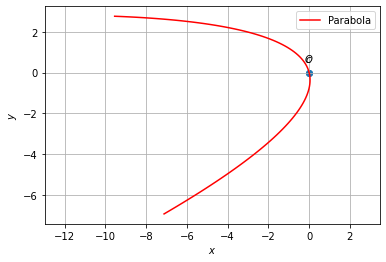
\includegraphics[width =\columnwidth]{solutions/41/1/parabola plot.png}
	\caption{Parabola }
	\label{eq:solutions/41/1/fig:1}
\end{figure}	

